\documentclass[12pt]{article}

\usepackage{amsmath}

\usepackage{graphicx}
\usepackage{pgfplots}
\usepackage{hyperref}
\usepackage{amsmath}
\usepackage{amssymb}

\usepackage[utf8]{inputenc}

\title{Algèbre Linéaire}

\author{Louis Gérard}

\date{Automne 2023}

\begin{document}

\maketitle

\newcommand{\R}{\mathbb{R}}
\newcommand{\K}{\mathrm{K}}
\newcommand{\C}{\mathbb{C}}
\newcommand{\zero}{\mathbb{0}}
\newcommand{\family}{\{v_i\}_{i\in I}}
\newcommand{\uv}{\{u,v\}}

Ce document est une tentative de polycopié pour le cours d'algèbre 
linéaire I d'automne 2023 11M010. Tous les exemples du cours n'y figurent pas, mais tout le reste y est (ou devrait y être).
\\
Si vous trouvez une erreur (il y en a), faites une pull request sur git si vous savez comment faire. Sinon, contactez-moi sur Telegram (alternis) 
Listes des cours inclus dans le document :
\begin{itemize}
    \item Cours du 21.9
\end{itemize}
\pagebreak
\tableofcontents
\pagebreak

\section*{Motivation}
On souhaite résoudre un système d'équations linéaires.
\subsection*{Exemple 1}
Une équation linéaire à 1 inconnue de la forme :
$$
ax+b=c
$$
Ici, $x$ est l'inconnue et $a,b,c \in \R$ des constantes. On souhaite trouver $Sol \subset \R$
l'ensemble des solutions.
$$
Sol = \begin{cases} \{\frac{c-b}{a}\}, \text{ si a} \neq 0 \\
     \R, \text{ si a}=0 \text{ et } b = c \\ 
    \emptyset, \text{ si a}=0 \text{ et } b \neq c
    \end{cases}
$$
\subsection*{Définition 1}
Un système à $m$ équations linéaires à $n$ variables à 
coefficients réels* est constitué de $m$ équations de la forme :

$$
\begin{aligned}
    a_{11}x_1 + a_{12}x_2 + \dots + a_{1n}x_n &=b_1 \\
    & \vdots \\
    a_{m1}x_1 + a_{m2}x_2 + \dots + a_{mn}x_n &=b_m \\
\end{aligned}
$$
Les coefficients du système sont $a_{11}, \dots, a_{1n}, \dots, a_{m1}, \dots, a_{mn}$.
On appelle les coefficients $b_1, \dots, b_m$ les "coefficients libres".
Dans le cas particulier où $b_1 = \dots = b_m$, on dit que le système est \textbf{homogène}.

\textit{*On parle aussi de systèmes à coefficients complexes. Ils sont abordés plus loin, dans le chapitre X.}

Résoudre un tel système revient à trouver son ensemble de solutions $Sol$.
$$Sol = \{(\alpha_1, \dots, \alpha_n) \text{ où } \alpha_i \in \R, i = 1, \dots, n\}$$
\pagebreak
\section{Chapitre 1 - Espaces vectoriels}
\subsection{Définitions, exemples et propriétés}
Pour motiver la définition, on considère quelques exemples de systèmes linéaires.
\subsubsection*{Exemple a)}
$n=2, m=2$
$$\begin{aligned}
\begin{cases}
    x+2y = 2 \\
    x-y=-4
\end{cases}
\\
x = -4+y \Rightarrow 3y = 6 \Rightarrow \begin{cases} y = 2 \\ x = -2 \end{cases}
\\
Sol = \{(-2, 2)\}
\end{aligned}
$$
Cette solution a un sens géométrique : les droites d'équations décrites dans le systèmes se croisent bien au point $(-2, 2)$.
\\
\begin{center}
    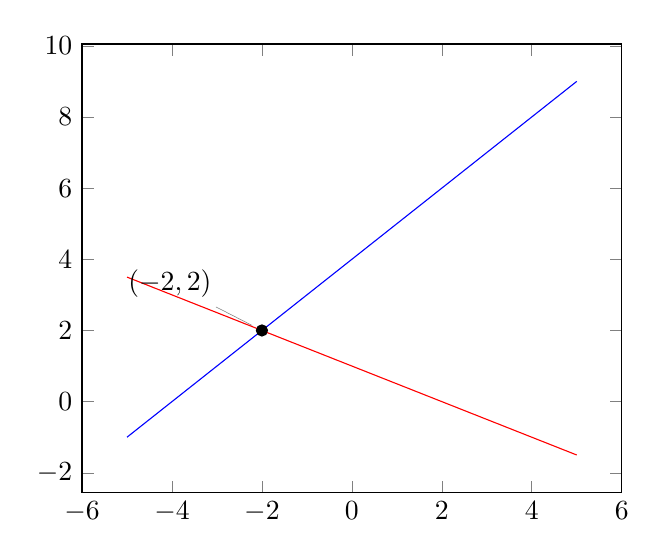
\begin{tikzpicture}
        \begin{axis}
        \addplot[color=red]{-0.5*x+1};
        \addplot[color=blue]{x+4};
        \addplot[mark=*] coordinates {(-2,2)} node[pin=150:{$(-2,2)$}]{} ;
        \end{axis}
        \end{tikzpicture}
\end{center}
\pagebreak
\subsubsection*{Exemple b)}
$n=2, m=2$
$$
\begin{cases}
    x+2y = 2 \\
    x+2y= 0
\end{cases} \Rightarrow Sol = \emptyset
$$
Les droites ne se croisent effectivement jamais.
\begin{center}
    \begin{tikzpicture}
        \begin{axis}
        \addplot[color=red]{1-0.5*x};
        \addplot[color=blue]{-0.5*x};
        \end{axis}
        \end{tikzpicture}
\end{center}
\pagebreak
\subsubsection*{Exemple c)}
$n=2, m=2$
$$
\begin{cases}
    x+2y = 0 \\
    2x+y= 0
\end{cases} \Rightarrow Sol = \{(0,0)\}
$$
Ce système est homogène. 
\begin{center}
    \begin{tikzpicture}
        \begin{axis}
        \addplot[color=red]{-0.5*x};
        \addplot[color=blue]{-2*x};
        \addplot[mark=*] coordinates {(0,0)} node[pin=150:{$(0,0)$}]{} ;
        \end{axis}
        \end{tikzpicture}
\end{center}
\pagebreak
\subsubsection*{Exemple d)}
$$
\begin{cases}
    x+2y=0
    \\
    2x+2y=0
\end{cases} \Rightarrow Sol = \{(x,y) \in \R^2 : y = - \frac{x}{2}\}
$$
\begin{center}
    \begin{tikzpicture}
        \begin{axis}
        \addplot[color=red]{-0.5*x};
        \addplot[color=blue]{-0.5*x};
        \end{axis}
        \end{tikzpicture}
\end{center}
Les deux droites sont superposées, l'ensemble des solutions prend donc la forme d'une droite.
\pagebreak
\subsubsection*{Exemple e)}
Ici, $m=3, n=2$.
$$
\begin{cases}
    x+2y = 0
    \\
    2x+y = 0
    \\
    x-y = 5
\end{cases} = \emptyset    
$$

\begin{center}
    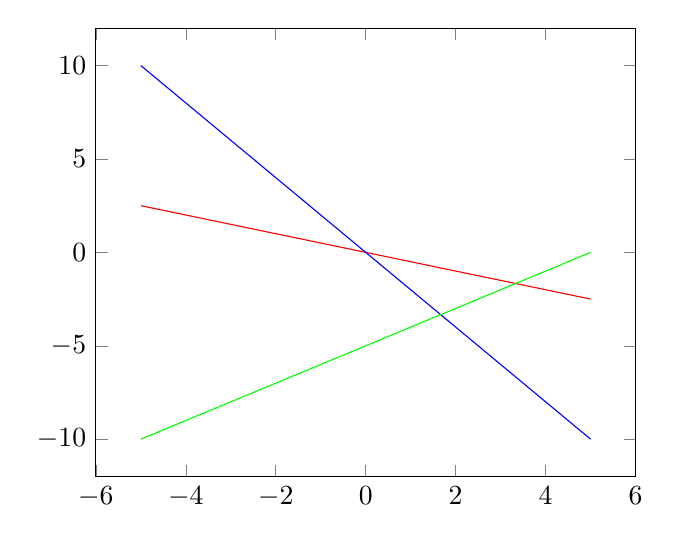
\begin{tikzpicture}
        \begin{axis}
        \addplot[color=red]{-0.5*x};
        \addplot[color=blue]{-2*x};
        \addplot[color=green]{x-5};
        \end{axis}
        \end{tikzpicture}
\end{center}
Il n'y a pas de solution, puisqu'il n'existe aucun point d'intersection des trois droites.

\pagebreak
\subsection{Propriétés des solutions de systèmes homogènes}
On observe que l'ensemble de solutions d'un système homogène à $m$ équations et $n$ inconnues satisfait les trois propriétés suivantes :
\begin{enumerate}
    \item $\alpha_1 = 0, \dots, \alpha_n = 0$ est toujours une solution.
    \item si $(\alpha_1, \dots, \alpha_n)$ et $(\alpha_1', \dots, \alpha_n')$ 
    sont deux solutions, alors leur somme $(\alpha_1+\alpha_1', \dots, \alpha_n+\alpha_n')$ est aussi une solution.
\end{enumerate}
\subsubsection{Démonstration de la propriété 2}
Soit $i \in \{1, \dots, m\}$.
$$\begin{aligned}
a_{i1}(\alpha_1+\alpha_1') + \dots + a_{in}(\alpha_n+\alpha_n')
\end{aligned}
$$
On a remplacé les facteurs $(x_1, \dots, x_n)$ par les solutions supposées.
Par distributivité, on obtient :
$$\begin{aligned}
    &a_{i1}\alpha_1 + a_{i1}\alpha_1' + \dots + a_{in}\alpha_n + a_{in}\alpha_n' \\
    &= (a_{i1}\alpha_{1}+a_{i2}\alpha_2+\dots+a_{in}\alpha_n) + (a_{i1}\alpha_{1}'+\dots+a_{in}\alpha_n') \\
    &= 0 
\end{aligned}
$$
Or, on sait déjà que $(\alpha_1, \dots, \alpha_n)$ et $(\alpha_1', \dots, \alpha_n')$ sont des solutions. On peut en conclure que leur addition donne également zéro, et que notre solution supposée $(\alpha_1 + \alpha_1', \dots, \alpha_n + \alpha_n')$ en est bien une.

On peut prouver la propriété 3) de la même façon.

\pagebreak
\subsection{Définition d'un espace vectoriel}
Un \textbf{espace vectoriel réel} est un ensemble $V$ muni de deux opérations :
\begin{enumerate}
    \item "addition" : $V \times V \rightarrow V, (v, v') \rightarrow v + v'$
    \item "multiplication par un scalaire" : $\R \times V \rightarrow V, (\alpha, v) \rightarrow \alpha \cdot v$ 
\end{enumerate}

Ces deux opérations doivent satisfaire une liste d'axiomes pour que l'ensemble soit un espace vectoriel.
\begin{itemize}
    \item $\forall u,w,u \in V$, on a $(u+w)+u=v+(w+u)$, l'associativité de l'addition.
    \item $\forall u,w \in V, v+w = w+v$, commutativité de l'addition
    \item Il existe un élément noté $\mathbb 0 \in V$ tel que $\mathbb 0 +v = v \quad \forall v \in V$    
    \item $\forall v \in V \space \exists -v : v + (-v) = \mathbb 0$
    \item $\alpha * (u+v) = \alpha*u+\alpha*v \space \forall \alpha \in \R, u,v \in V$
    \item $(\alpha + \beta) * v = \alpha * v + \beta * v \space \forall \alpha, \beta, \in \R, v \in V$, distributivité de l'addition dans $\R$
    \item $(\alpha*\beta)*v=\alpha*(\beta*v)$, associativité de la multiplication dans $\R$ par un scalaire.
    \item $1 \in R : 1*v=v \quad \forall v \in V$ 
\end{itemize}

On appelle les éléments de l'espace vectoriel $V$ des \textbf{vecteurs} et les éléments du corps $K$ sur le quel $V$ est défini des \textbf{scalaires}.
\end{document}